%%%%%%%%%%%%%%%%%%%%%%%%%%%%%%%%%%%%%%%%%
%
% Optics and Radar -based observations
% EISCAT Space Weather Practical
%
%%%%%%%%%%%%%%%%%%%%%%%%%%%%%%%%%%%%%%%%%

%----------------------------------------------------------------------------------------
%	DOCUMENT CONFIGURATIONS
%----------------------------------------------------------------------------------------

\documentclass{article}

\title{\textbf {Optics and Radar Based Observations} \\ Practical\\ EISCAT ESR - incoherent scatter and weather in space} % Title
\def\authorivan{Ivan \v Sinkarenko}
\def\authoranu{Anuraj Rajendraprakash}
\author{\authorivan\\\authoranu}

\usepackage{graphicx}
\usepackage{fullpage}
\usepackage{url}
\usepackage{caption}
\usepackage{subcaption}

\begin{document}

\maketitle % Insert the title, author and date

\centerline{Referee: Dr. Victoria Barabash}

\setlength\parindent{0pt} % Removes all indentation from paragraphs

\renewcommand{\labelenumi}{\alph{enumi}.} % Make numbering in the enumerate environment by letter rather than number (e.g. section 6)
\clearpage

\tableofcontents

\listoffigures

\clearpage

%----------------------------------------------------------------------------------------
%	SECTION 1. Introduction
%----------------------------------------------------------------------------------------

\section{Introduction}
Space weather is the concept of changing environmental conditions in near-Earth space or the space from the Sun's atmosphere to the Earth's atmosphere. The observation of space weather is done both for scientific research and for applications. The type of observation done for science has varied over the years as the frontiers of our understanding has increased and due to competition for resources from other types of space-related research. The observations related to applications have been more systematic and has expanded over the years as awareness and applications have increased. \cite{Wiki:2012sw}\\
One of the ways to understand influence of space weather on near-Earth environment is to study ionosphere using incoherent scatter radar. A radar beam scattering off electrons in the ionospheric plasma creates an incoherent scatter return. The distribution function of the ionospheric electrons is modified by the much slower and massive positive ions — electron density fluctuations relate to ion temperature, mass distribution, and motion. The incoherent scatter signal allows measurement of electron density, ion temperature and electron temperatures, ion composition and plasma velocity. \cite{Wiki:2012is}
\\
The purpose of this laboratory experiment is to get acquainted with the EISCAT Svalbard Radar (ESR) system operating at frequency of 500 MHz. The transmitter/receiver of ESR is situated in Longyearbyen, Svalbard at 78$^{\circ}$09'11" N, 16$^{\circ}$01'44" E. Radar system has been run remotely with assistance from EISCAT staff. The main objective of the experiment is to understand how the ESR system works, which physical parameters can be studied in the data analysis and to compare the obtained results with space weather observations from other sources. \cite{Barabash:2011esr}

%----------------------------------------------------------------------------------------
%	SECTION 2. Experiment
%----------------------------------------------------------------------------------------

\section{Experiment}

The ESR is controlled by the EISCAT Realtime Operating System (EROS). This particular experiment comes with a codename "Beata".\\
The experiment took place at space campus near Kiruna, Sweden between 11:45 UT and 12:15 UT.
List of used commands during the experiment:
\begin{itemize}
\item \textbf{runexperiment /kst/exp/exp1 time now exp1}: (the full path must be given) at time time, which can be given at as \emph{HH:MM:SS} or \emph{now} or \emph{fullminute} etc.
\item \textbf{enablerecording}: Start recording data.
\item \textbf{disablerecording}: Stop recording data.
\item \textbf{stopexperiment}: Stop experiment immediately.
\end{itemize}
During the experiment data has been observed in real time with help of the real time graph software \emph{rtg}. Later on, raw data was collected from the EISCAT servers and used for "GUISDAP" Matlab script to compute final measurement data.

%----------------------------------------------------------------------------------------
%	SECTION 3. Data analysis and discussion
%----------------------------------------------------------------------------------------

\section{Data analysis and discussion}

After the experiment was performed the information about space weather was retrieved from the different sources. It was necessary to collect the relevant information from other sources to ensure that the experiment didn't go wrong and the data acquired is meaningful. For this reason Internet resources were used, including:
\begin{itemize}
\item \url{http://sohowww.nascom.nasa.gov/}
\item \url{http://www.swpc.noaa.gov/ace}
\item \url{http://www.spaceweather.com/}
\item \url{http://www.spacew.com/}
\end{itemize}
Later the data was combined to form the single impression of current space weather, including various solar wind parameters, sunspot number, magnetic field and plasma parameters.\\
\\
\textbf{Space weather for 2015-05-15 12:31 UT}:\\
\begin{tabular}{ l l }
Solar Wind speed:              & 396.2 $km/s$         \\
Solar Wind temperature:        & 42421.5 $K$          \\
Solar Wind density:            & 2.1 $particles/cm^3$ \\
Solar Wind pressure:           & 0.6 $nPa$            \\
Sunspots number:               & 72                   \\
Total Magnetic Field, B:       & 7.6 $nT$             \\
B-Field in x-direction, $B_x$: & 2.6 $nT$             \\
B-Field in y-direction, $B_y$: & -5.4 $nT$            \\
B-Field in z-direction, $B_z$: & 4.6 $nT$             \\
Latitude angle, $\beta$:       & 37.5$^{\circ}$       \\
Angle, $\theta$:               & 52.5$^{\circ}$       \\
\end{tabular}
\\
\\
\\
Also images were collected from different instruments of SOHO spacecraft, which made it clear that there were no any significant solar flares which could affect measurements at that time. The pictures are shown in Figure \ref{fig:SOHO}.

\begin{figure}[h!tb]
	\centering
	\begin{subfigure}[b]{0.16\textwidth}
		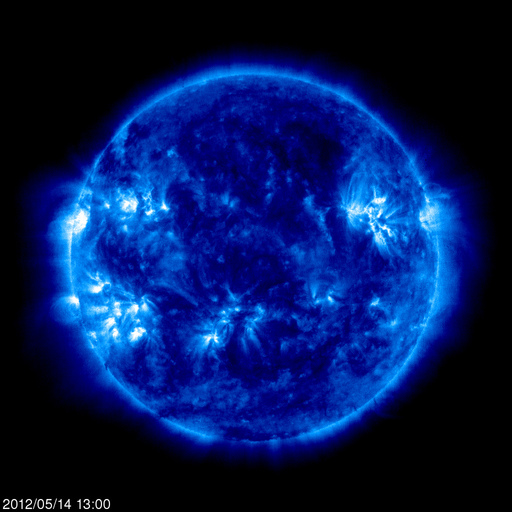
\includegraphics[width=\textwidth]{Figures/SOHOEIT171.jpg}
		\caption{EIT 171}
		\label{fig:SOHOEIT171}
	\end{subfigure}
	\begin{subfigure}[b]{0.16\linewidth}
		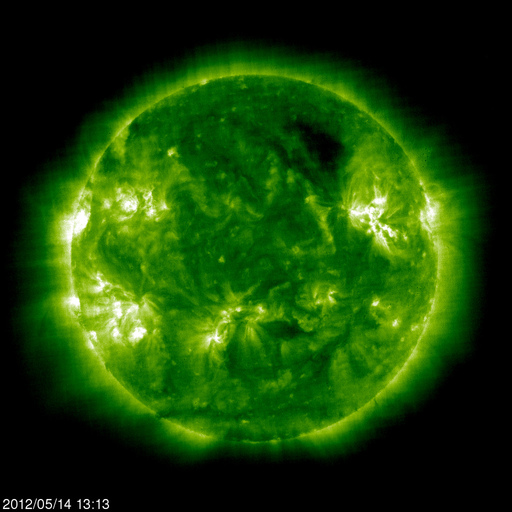
\includegraphics[width=\textwidth]{Figures/SOHOEIT195.jpg}
		\caption{EIT 195}
		\label{fig:SOHOEIT195}
	\end{subfigure}
	\begin{subfigure}[b]{0.16\linewidth}
		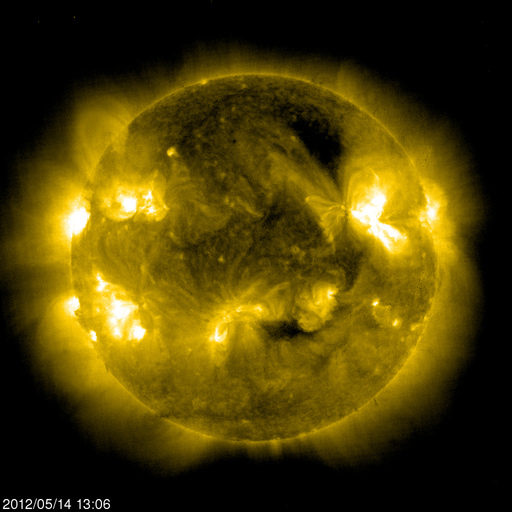
\includegraphics[width=\textwidth]{Figures/SOHOEIT284.jpg}
		\caption{EIT 284}
		\label{fig:SOHOEIT284}
	\end{subfigure}
	\begin{subfigure}[b]{0.16\linewidth}
		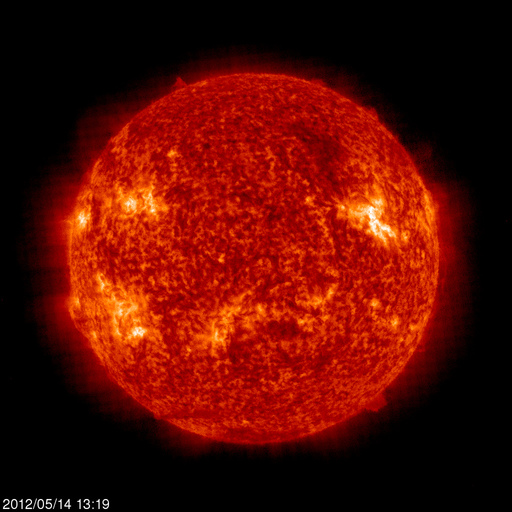
\includegraphics[width=\textwidth]{Figures/SOHOEIT304.jpg}
		\caption{EIT 304}
		\label{fig:SOHOEIT304}
	\end{subfigure}
	\begin{subfigure}[b]{0.16\linewidth}
		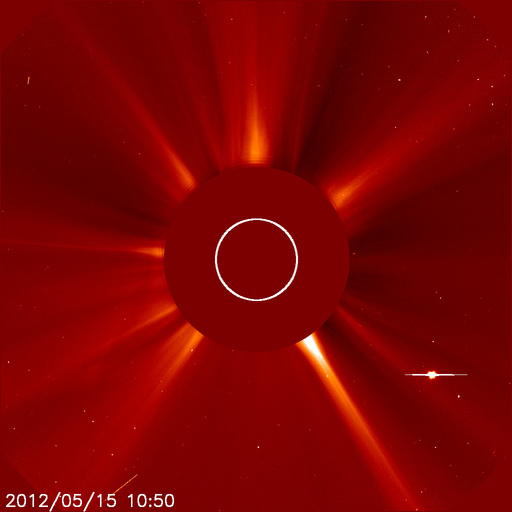
\includegraphics[width=\textwidth]{Figures/SOHOLASCOC2.jpg}
		\caption{LASCO C2}
		\label{fig:SOHOLASCOC2}
	\end{subfigure}
	\begin{subfigure}[b]{0.16\linewidth}
		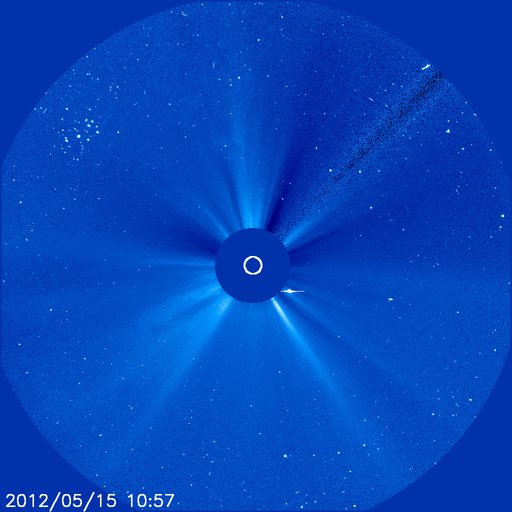
\includegraphics[width=\textwidth]{Figures/SOHOLASCOC3.jpg}
		\caption{LASCO C3}
		\label{fig:SOHOLASCOC3}
	\end{subfigure}
	\caption{SOHO instrument images}
	\label{fig:SOHO}
\end{figure}

In the next step, the International Reference Ionosphere (IRI) model was retrieved from the website \url{http://iri.gsfc.nasa.gov}. The time and the coordinates of the experiment were entered for this model. The vertical profile of the electron number density according to IRI model is plotted in Figure \ref{fig:iri}.
\begin{figure}[h!tb]
	\centering
	\begin{minipage}[t]{0.45\linewidth}
		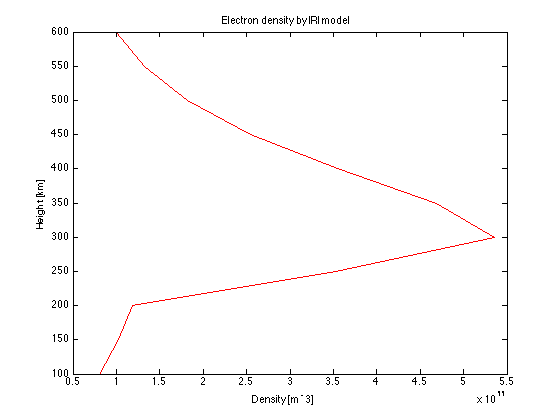
\includegraphics[width=\textwidth]{Figures/iri.png}
		\caption{Electron density from IRI model.}
		\label{fig:iri}
	\end{minipage}
	\begin{minipage}[t]{0.45\linewidth}
		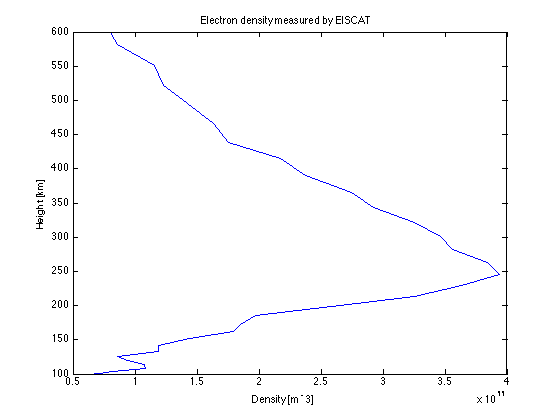
\includegraphics[width=\textwidth]{Figures/density.png}
		\caption{Uncalibrated density from ESR measurements.}
		\label{fig:density}
	\end{minipage}
\end{figure}
The real measurements from ESR were got by running "GUIDSDAP" script, which created a bunch of *.mat files. All these files had number densities for the same height which were slightly different. Although altitude data also was not the same among the files, the difference was just tens of meters. It was decided to average measurements by taking mean values of altitudes as well as number densities. In the end, the vertical profile of averaged electron number density $N_e$ was plotted, as shown in Figure \ref{fig:density}.\\
Comparing two electron number density signatures yields to the conclusion that, even though the shapes of the densities are similar, they have quite a big difference. It is seen that maximum electron number density in IRI model occurs at approximately 300 km altitude, whereas in EISCAT measurements it is just slightly less than 250 km. Moreover, EISCAT maximum electron number density is $3.936*10^{11}\:m^{-3}$, while IRI model show around $5.35*10^{11}\:m^{-3}$. Such a behavior makes it clear that ESR data is not calibrated.\\
\\
One more way to ensure that the data needs to be calibrated is to compare electron number density with the one from another source, for instance, dynasonde. Dynasonde is an ionosonde competent to measure the dynamics of the ionosphere. \cite{Ngdc:2004d} An ionosonde is a special radar for the examination of the ionosphere. The transmitter sweeps all or part of the HF frequency range, transmitting short pulses. These pulses are reflected at various layers of the ionosphere, at heights of 100-400 km, and their echos are received by the receiver and analyzed by the control system. The result is displayed in the form of an ionogram, a graph of reflection height (actually time between transmission and reception of pulse) versus carrier frequency. \cite{Wiki:2012i} EISCAT runs its own dynasonde, which among all other values provided has $f_0F2$ coefficient. $f_0F2$ is related to electron number density $N_e$ as described in Equation \ref{eq:f0f2}
\begin{equation}
\label{eq:f0f2}
f_0F2=\frac{\sqrt{\frac{N_e\,e^2}{\epsilon_0\,m_e}}}{2\pi}
\end{equation}
where $N_e$ is electron number density, $\epsilon_0$ is electric constant, $e$ is electron charge and $m_e$ is electron mass.\\
\\
Using this equation electron number densities were calculated from the dynasonde data and maximum value has been found: $5.634512*10^{11}\:m^{-3}$. This value has a 30.2\% difference with $3.936*10^{11}\:m^{-3}$, which has been derived earlier from the ESR measurements. According to EISCAT guidelines, if the values differ from each other more than 10\% the electron number density profile should be calibrated. Calibration is performed by defining a Magic constant. The Magic constant has been introduced and agreed by EISCAT HQ in order to take into account the effect of external environment on the transmitted power, i.e. snow on the antenna etc. The Magic constant is a scale factor for the real radar constant. \cite{Barabash:2011esr} It is calculated from Equation \ref{eq:mag_cnst}.
\begin{equation}
\label{eq:mag_cnst}
Magic\_const=\frac{N_{e_{dynasonde}}}{N_{e_{EISCAT}}}
\end{equation}
Given the values, Magic constant was calculated and added to "GUISDAP" Matlab script as a parameter "Magic\_const = 1.431642". Once calibrated data was got, all the above steps were applied for it. The resulting electron number density plot is shown in Figure \ref{fig:density_cal}.
\begin{figure}[h!tb]
		\centering
	\begin{minipage}[t]{0.45\linewidth}
		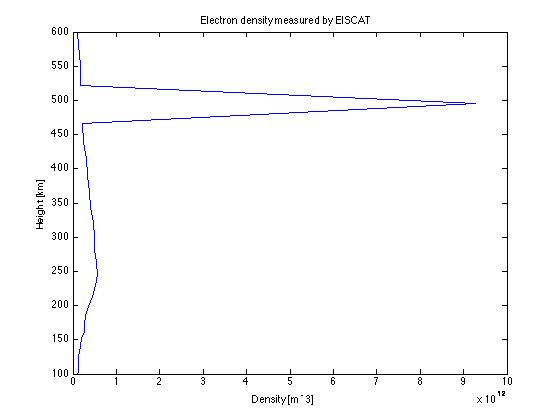
\includegraphics[width=\textwidth]{Figures/density_cal.png}
		\caption{Calibrated density from ESR measurements with spikes.}
		\label{fig:density_cal}
	\end{minipage}
	\begin{minipage}[t]{0.45\linewidth}
		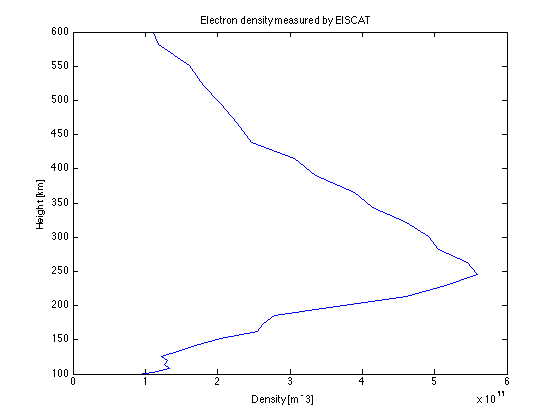
\includegraphics[width=\textwidth]{Figures/density_cal_no_spikes.png}
		\caption{Calibrated density from ESR measurements without spikes.}
		\label{fig:density_cal_no_spikes}
	\end{minipage}
\end{figure}
This graph contains very long spike at altitude of 500 km which is not common. One possible explanation is that during the experiment an object with high reflective properties entered the field view of the radar. Actually, EISCAT assistant mentioned once that there was a spacecraft crossing studied area during the experiments. However, uncalibrated data did not contain such an enormous anomaly in measurements. Thus, the reason is still remaining uncertain. To continue data interpretation, condition was inserted to eliminate such spikes. Basically, if it detects variations larger than factor of 10, it takes a mean value of two adjacent density values. The vertical profile of calibrated electron densities with spikes removed is shown in Figure \ref{fig:density_cal_no_spikes}. The maximum number density with this data is $5.590073*10^{11}\:m^{-3}$, which is different from the maximum density calculated using $f_0F2$ coefficient only by 0.8\%. The calibrated and refined density profile also was compared with IRI model profile as shown in Figure \ref{fig:iri_eiscat}. This time data match is much more accurate. It proves that calibration using Magic constant is accurate enough and the calibrated data is reliable. However, profiles are still not perfectly similar. This can happen because of several reasons, for example, snow lying on the radar dish. The small downward shift could be caused by an active electric field present in the ionosphere. \cite{Stoffregen:1969ed} Also for the altitudes below 300 km there is bigger downward shift which might be caused by reflection because of the presence of a wave in the solar wind, however this is not likely, because investigation of the space weather showed that there were no strong solar flares during the relevant time period.
\begin{figure}[h!tb]
	\centering
	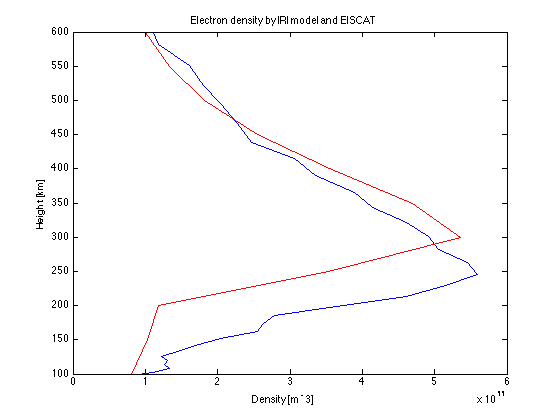
\includegraphics[width=0.5\textwidth]{Figures/iri_eiscat.png}
	\caption{Calibrated density from ESR measurements (blue) and IRI model (red).}
	\label{fig:iri_eiscat}
\end{figure}


%----------------------------------------------------------------------------------------
%	SECTION 4. Conclusion
%----------------------------------------------------------------------------------------

\section{Conclusion}

%----------------------------------------------------------------------------------------
%	SECTION 5. REFERENCES
%----------------------------------------------------------------------------------------
\newpage
\begin{thebibliography}{9}

\bibitem{Wiki:2012sw}
Wikipedia.org. (2012).
\newblock {\em Space weather}.
\newblock {\url{http://en.wikipedia.org/wiki/Space_weather}}.

\bibitem{Wiki:2012is}
Wikipedia.org. (2012).
\newblock {\em Incoherent scatter}.
\newblock {\url{http://en.wikipedia.org/wiki/Incoherent_scatter}}.

\bibitem{Barabash:2011esr}
EISCAT HQ / Barabash V. (2011).
\newblock {\em Practical. EISCAT ESR - incoherent scatter and weather in space}.
\newblock Lule\aa \ University of Technology, Kiruna, Sweden.

\bibitem{Wiki:2012i}
Wikipedia.org. (2012).
\newblock {\em Ionosonde}.
\newblock {\url{http://en.wikipedia.org/wiki/Ionosonde}}.

\bibitem{Ngdc:2004d}
National Geophysical Data Center (NGDC) (2004).
\newblock {\em What is a Dynasonde?}.
\newblock {\url{http://www.ngdc.noaa.gov/stp/IONO/Dynasonde/whatis.htm#Dynasonde}}.

\bibitem{Stoffregen:1969ed}
W. Stoffregen (1969).
\newblock {\em Electron density variation observed in the E-layer below an artificial barium cloud}.
\newblock {Uppsala Ionospheric Observatory, Research Institute of Swedish National Defence, Uppsala, Sweden}.

\bibitem{Skolnik:2001irs}
Skolnik M. ~I.  (2001).
\newblock {\em Introduction to Radar Systems}.
\newblock The McGraw-Hill Companies, Inc., New York, United States.

\bibitem{Rottger:2000ip}
R\"ottger J.  (2000).
\newblock {\em The Instrumental Principles of MST Radars and Incoherent Scatter Radars and The Configuration of Radar System Hardware}.
\newblock Max Planck Institut F\"ur Aeronomie, Katlenburg-Lindau, Germany.


\end{thebibliography}

%----------------------------------------------------------------------------------------
%	SECTION 6. Confirmation
%----------------------------------------------------------------------------------------
\newpage
\section{Confirmation of Participation}

This is to confirm that the members of this team participated on the investigation of the required information to solve the assignment, generated their code to perform the calculation and discussed the results.\\
\vspace{2cm}
\newline
\line(1,0){200}\\
\authorivan\\
\vspace{2cm}
\newline
\line(1,0){200}\\
\authoranu\\


\end{document}